% A workaround to allow relative paths in included subfiles
% that are to be compiled separately
% See https://tex.stackexchange.com/questions/153312/subfiles-inside-a-subfile-using-relative-paths
\providecommand{\main}{..}
\documentclass[\main/thesis.tex]{subfiles}

\begin{document}

\chapter{Matrix Math Assist}
\label{cha:mma}

\Gls{power10}'s \gls{mma} is what is being called a ``matrix engine''~\autocite{domke2020matrix}.
\todo{Waiting for actual publication of matrix engine paper from IPDPS instead of the arxiv preprint.}
Specifically, it is a facility in the \gls{cpu} whose function is computing matrix multiplication.
Matrix engines have appeared in multiple architectures, though their implementation and design choices differ.
Likewise, the algorithm for optimally making use of each of these architectures differs.
While this work focuses on \gls{mma}, a discussion of the differences in these architectural implementations follows in \rsec{matrixEngines}.

\section{Computation Style}
\label{sec:compuationStyle}

\begin{figure}[t]
 \begin{subfigure}{.45\linewidth}
   \centering
   \begin{tikzpicture}[scale=1/2]
     \draw[step=1, shift={(0, 3)}] (0, 0) grid +(4, 1);
     \node at (4.75, 2) {$\times$};
     \draw[step=1, shift={(5.5, 0)}] (0, 0) grid +(1, 4);
     \node at (7.25, 2) {$=$};
     \draw[step=1, shift={(8, 3)}] (0, 0) grid +(1, 1);
     \node at (2, 5) {$A$};
     \node at (6, 5) {$B$};
     \node at (8.5, 5) {$C$};
   \end{tikzpicture}
   \caption{Inner product.}
   \label{fig:innerProduct}
 \end{subfigure}
 \hfill
  \begin{subfigure}{.45\linewidth}
    \centering
    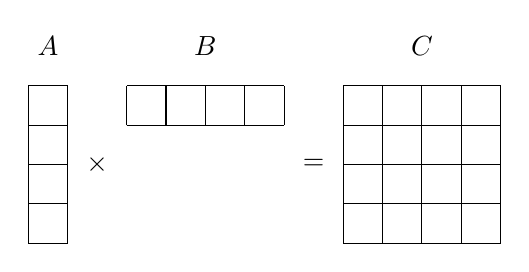
\begin{tikzpicture}[scale=1/2]
      \draw[step=1, shift={(0, 0)}] (0, 0) grid +(1, 4);
      \node at (1.75, 2) {$\times$};
      \draw[step=1, shift={(2.5, 3)}] (0, 0) grid +(4, 1);
      \node at (7.25, 2) {$=$};
      \draw[step=1, shift={(8, 0)}] (0, 0) grid +(4, 4);
      \node at (.5, 5) {$A$};
      \node at (4.5, 5) {$B$};
      \node at (10, 5) {$C$};
    \end{tikzpicture}
  \caption{Outer-product (rank-$1$ update) operation.}
    \label{fig:outerProduct}
  \end{subfigure}
  \hfill
  \caption{Example matrix-matrix computation styles.}
  \label{fig:product}
  \vspace{-0.15cm}
\end{figure}

\Gls{mma}'s design is built around the choice to compute the \emph{outer product} instead of the inner product, the operation that usually first comes to mind when discussing matrix multiplication.
Both operations arrive at the same destination albeit via different processes.
Consider \rfig{product}.
\rfig{innerProduct} illustrates the inner product: an element-wise multiplication between a row of matrix $A$ and a column of matrix $B$ followed by the summation of the products (\ie the dot product).
In short, two vectors produce a single, fully-computed output element.
Computing the outer product, shown in \rfig{outerProduct}, results in a column of matrix $A$ and a row of matrix $B$ producing a \emph{partial} output matrix.
That is, a matrix whose elements are the result of a single product.
One such matrix is produced per combination of $A$ column and $B$ row; these matrices must be summed to produce the output $C$.

At the end of the computation, both methods will have performed exactly the same number of multiplications and additions.
As well, in a machine with unlimited resources, including vector registers of unlimited length, they will have performed the same number of stores and loads.
In such a theoretical framework, at least in terms of computations performed, neither method can be said to be better.
However, in a practical machine, it is impossible to load the entirety of a long row or of a long column into vector registers in order to fully compute a portion of the matrix.
\nelson{This}
This makes tiling a necessity.
Tiling, as discussed in \todo{reference mat mul section}, breaks the operation into smaller, more manageable operations.
Different methods of tiling will affect the overall number of loads and stores performed as well as the latencies of these loads and stores based on properties of the memory hierarchy.
Thus, how these load and store operations interact with the memory hierarchy and register usage is the largest differentiating factor between the two methods.

Goto and van de Geijn~\autocite{goto2008anatomy} demonstrate that large matrix-matrix multiplications based on the dot-product approach are inferior in this regard.
\todo{Make sure that Goto's work has been adequately explained in mat mul section for the rest of the paragraph.}
For a dot-product solution, a packed version of $C$ is made resident in L2 cache.
Because tiling necessitates an accumulation step, the values of $C$ are both read and written for each iteration over a tile.
\nelson{This}
This is in contrast to 
\nelson{Why "non-dot-product methods" instead of the outer-product approach? Are there other non-dot-product methods that we should also consider?}
non-dot-product methods which choose to pack and make resident either $A$ or $B$ in L2 cache.
\nelson{I do not understand the reasoning here. How does the conclusion "the dot product requires twice as much bandwidth" follows from the premise that "$A$ and $B$ are read-only"? Maybe you have to mention that when $C$ is stored in L2 it must be read and written? Is that the reason? Avoid using "Since" because of its temporal meaning. In this case you can use "Given that"}
Since $A$ and $B$ are read-only, the dot product requires twice as much of the expensive L2 bandwidth when compared with other methods.

On the micro scale, the dot-product approach also makes poor use of \gls{simd} capabilities.
Computing he dot product requires a horizontal reduction: the reduction of all the lanes of a vector register into a single scalar element.
\nelson{"the territory of \gls{simd}" sounds colloquial and not very precise. How is such territory defined?}
Computing a partial result in this manner effectively leaves the territory of \gls{simd} and creates a scalar value.
The outer product, however, uses a vertical reduction (or element-wise reduction) that allows all values to be accumulated in-place within the destination vector register or, in the case of \gls{mma}, the destination accumulator register.

It is for these reasons that \gls{hpc} libraries implement matrix-matrix multiplication by emulating the outer product where only inner product operations are available.
\nelson{This}
This is possible by broadcasting (duplicating) a single value from one operand matrix into all elements of a vector register and then multiplying that vector with a full vector from the other operand.
\Gls{mma} eschews this technique by directly providing outer product capabilities, removing unnecessary overhead.

\section{Architecture}
\gls{mma} adds a new architectural feature: eight accumulator (ACC) registers.
Accumulators and the new instructions for interacting with them enable the efficient matrix-matrix multiplication outlined above.
\nelson{What "this information" refers to?}
Much of this information can be found throughout the \gls{power10} \gls{isa} document though some of it comes as insight from engineers at \gls{ibm} or external sources.
\bk{Unsure if I should drop the previous sentence.}

\subsection{Accumulator Assembly and Disassembly}
\bk{Should I use ACC or accumulator throughout the rest of the work?}
\nelson{You can pick between them as appropriate. I prefer "accumulator" in the middle of a sentence and "ACC[0]" or so when referring to a specific one.}
An accumulator, in all interactions with \gls{mma}, can be thought of as a single register consisting of $4 \times 4$ 32-bit elements.
Accumulators may be assembled (initialised) in three manners:
\begin{enumerate*}[itemjoin*={{ and }}, label=\textbf{(\arabic*)}, after={.}]
  \item set to zeroes (\code{xxsetaccz}, Set Acc to Zero)
  \item constructed from four consecutive VSRs (\code{xxmtacc}, Move To Acc)
  \item a multiplication instruction that does not accumulate (see \rsec{matMulMMA})
\end{enumerate*}
When constructing from VSRs, each VSR is moved into the ACC and becomes one row\footnotemark of the resulting accumulator.
\footnotetext{Viewing the vectors as rows is intuitively convenient, but relatively arbitrary in reality. See \rsec{arbitraryOrder} for use as columns.}

In its current iteration, accumulator $n$ is the logical grouping of four 128-bit VSRs (\code{VSR[4n:4n+3]}) into a single register.
As such, the four underlying registers used to construct the accumulator are unavailable for use while the accumulator is in an assembled state.
For example, \code{VSR[0:3]} are unavailable while \code{ACC[0]} is assembled.
This blocking effect also applies to the underlying registers when assembling an accumulator to zeroes.

Blocking registers is viewed as a reasonable restriction in \gls{power10}.
However, the ISA is written such that if, in future versions of the hardware, the blocking restriction is removed, no changes will need to be made to the \gls{isa}.

The reverse operation to assembly is disassembly (\code{xxmfacc}, Move From Acc).
Disassembly moves each row from the accumulator into the same vector registers used for construction.
Therefore, as before, the first row of \code{ACC[0]} is placed into \code{VSR[0]}, the second row is placed into \code{VSR[1]}, \etc.

\subsection{Matrix Multiplication in MMA}
\label{sec:matMulMMA}

\begin{table}[t]
  \centering
  \begin{tabular}{| c | c | c | c | c |}
    \hline
    Instruction & Input Type & Output Type & Input Dim. & Smallest Computation \\\hline
    \code{xvi4ger8}  & \code{i4}     & \code{i32}    & $4 \times 8$ & \matmul{4}{8}{4} \\\hline
    \code{xvi8ger4}  & \code{i8}     & \code{i32}    & $4 \times 4$ & \matmul{4}{4}{4} \\\hline
    \code{xvi16ger2} & \code{i16}    & \code{i32}    & $4 \times 2$ & \matmul{4}{2}{4} \\\hline
    \code{xvf16ger2} & \code{half}   & \code{float}  & $4 \times 2$ & \matmul{4}{2}{4} \\\hline
    \code{xvbf16ger2} & \code{bfloat16}\footnotemark & \code{float}  & $4 \times 2$ & \matmul{4}{2}{4} \\\hline
    \code{xvf32ger}  & \code{float}  & \code{float}  & $4 \times 1$ & \matmul{4}{1}{4} \\\hline
    \code{xvf64ger}  & \code{double} & \code{double} & $4 \times 1$ & \matmul{4}{1}{2} \\\hline
  \end{tabular}
  \caption[MMA Instruction Description]{A description of \gls{mma} instructions investigated. Input dimension is transposed for second argument.}
  \label{tab:mmaInsts}
\end{table}
\footnotetext{Google's Brain floating point format~\autocite{wang2019bfloat16}.}

Assembly and disassembly delimit the lifetime of an accumulator, but the majority of its usage is found in matrix multiplication instructions.
\rtab{mmaInsts} shows all seven of the datatypes usable with \gls{mma}.
Instructions are given three arguments: an accumulator and two VSRs.
Considering the simplest example, single-precision floating point, a single four-element row or column fills the entire VSR ($32\text{bits} \times 4 = 128\text{bits}$).
This computation, \matmul{4}{1}{4}, is what is known as a \emph{rank-1 update} where one is the length of the innermost dimension.

Halving the size of the type to 16 bits means the argument VSRs are underutilised at half capacity.
Accumulators cannot be expanded and are always $4 \times 4$ matrices of 32-bit elements.
Thus, to increase utilisation of VSRs, the number of elements contained in each VSR is doubled resulting in doubling the number of rows or columns in a VSR.
Therefore, when using 16-bit values, the calculation performed is \matmul{4}{2}{4}, essentially computing two outer products at once (rank-2 update).
The same logic applies for eight- and four-bit types, computing rank-4 and rank-8 updates.

\subsubsection{Instruction Variants}

\begin{table}[t]
  \centering
  \begin{tabular}{| c | c | c |}
    \cline{2-3}
    \multicolumn{1}{c|}{} & \code{-p} & \code{-n}\\\hline
    \code{p-} & $C' = C + AB$ & $C' = -C + AB$\\\hline
    \code{n-} & $C' = C - AB$ & $C' = -C - AB$\\\hline
  \end{tabular}
  \caption[MMA Accumulation Suffix Computations]{MMA accumulation computations by instruction suffix. $C$ is the accumulator before accumulation while $C'$ is the accumulator after accumulation.}
  \label{tab:accSign}
\end{table}

An instruction without a suffix (first column of \rtab{mmaInsts}) will both assemble the given accumulator and overwrite it with the outer product of the two VSRs.
Afterward, to accumulate into the accumulator, each datatype has a ``family'' of instructions offering different semantics.
Four instruction suffixes are available: \code{pp}, \code{pn}, \code{np}, \code{nn}.
The \code{p} and \code{n} stand for positive and negative respectfully.
The first character specifies the sign of multiplication (\ie $\pm AB$) while the second specifies the sign of the accumulator (\ie $\pm C$).
The possible computations are shown in \rtab{accSign}.
Computations with 16-bit integers have an additional suffix, \code{s}, which replaces the regular overflow semantics with saturating semantics (\eg $0\text{xFFFF} + 1 = 0\text{xFFFF}$).
\bk{Should I describe saturating better?} \nelson{no need}

\nelson{this}
Beyond this, a single prefix exists: \code{pm}.
This prefix indicates a ``prefixed masked'' instruction.
These instructions take an extra three arguments, each of which is a mask that enables fine-grain control over the accumulation.
Each of the masks allows disabling of one of the following:
\begin{enumerate*}[itemjoin*={{ or }}, label=\textbf{(\arabic*)}, after={.}]
  \item any of the rows of the accumulation
  \item any of the columns of the accumulation
  \item any of the ranks of the accumulation
\end{enumerate*}
\nelson{This}
This disables only the application of these values to the accumulator, not the calculation; therefore, the execution time of a masked instruction is the same as that of an unmasked one.

\subsubsection{Double Precision Differences}
\label{sec:doubles}
When all other computations produce a 32-bit value, essentially gaining precision or remaining at the same precision, it would be unreasonable to force computations with 64-bit values to lose precision.
Therefore, when working with double-precision floats, accumulators become $4 \times 2$ arrays rather than the usual $4 \times 4$.
The change in data size affects the argument VSRs as well.
\nelson{Why "may"?}
A single VSR may now fit only two values.
Thus, in order to compute a rank-1 update, the first dimension requires four values, spread across two registers, while the second dimension now requires two values in a single register.

\section{Matrix Engine Comparison}
\label{sec:matrixEngines}

\nelson{I feel that the writing in this section could be improved.}

\nelson{"exists" where?}
Currently, there exists three relevant matrix engines but, given the current importance placed on matrix multiplication, it is unlikely that this list remains small.
Furthermore, each of the architectures have been designed in their own way with extensibility in mind implying that the richness and diversity of features is sure to improve as well.
\nelson{"landscape" is casual}
The current matrix engine landscape is summarised in \rtab{featComp}.

\begin{table}
  \centering
  \begin{tabular}{| c | c | c | c | c |}
    \hline
    Architecture & Location & \parbox[t][28pt][t]{40pt}{\centering Product Style} & Arg/Dest & Supported Types\\\hline
    \parbox[t][][t]{40pt}{\centering Power10 MMA} & core & outer & VSR/ACC & \parbox[t][40pt][t]{3.2cm}{\raggedright\code{i4}, \code{i8}, \code{i16}, \code{bfloat16}, \code{half}, \code{float}, \code{double}}\\\hline
    x86 AMX & off-core & inner & Tile &\parbox[t][11pt][t]{3.3cm}{\raggedright\code{i8}, \code{bfloat16}}\\\hline
    \parbox[t][][t]{60pt}{\centering ARM Neon/SVE} & core & inner & Vector register & \parbox[t][25pt][t]{3.3cm}{\raggedright\code{i8}, \code{bfloat16}, \code{float}, \code{double}}\\\hline
  \end{tabular}
  \caption[Matrix Engine Feature Comparison]{Comparison of features currently offered by cpu-based matrix engines.}
  \label{tab:featComp}
\end{table}

Matrix multiplication is a dedicated focus of x86's \gls{amx}.
The extension is implemented as an off-core accelerator with its own register file.
These new registers, called ``tiles'', are $16 \times 64$ bytes large.
Eight of these tiles are used as both argument and result registers in inner-product computations.
While it supports less types than \gls{mma}, it does supports two important types for artificial-intelligence workloads: \code{i8} and \code{bfloat16}.

In ARM's Neon and \gls{sve}, matrix multiplication is a small part of a larger vector extension.
It is thus implemented on-core as part of the regular vector facilities, much like \gls{mma}.
Like \gls{mma} as well, the architecture's regular vector registers are used as input.
However, these registers are passed to an inner-product computation whose destination is not a specialsed accumulator, just another regular vector register.
Neon, like \gls{amx}, supports \code{i8} and \code{bfloat16} while \gls{sve} adds support for \code{float} and \code{double}.
\end{document}
